%CHKTEX-FILE 46

\section*{SOAR Hardware Description}%
\label{sec:annex-OPL}
% In this section briefly describe the software and hardware of the robot

\setlength\intextsep{0pt}
\begin{wrapfigure}[10]{r}{0.3\textwidth}
	\centering
	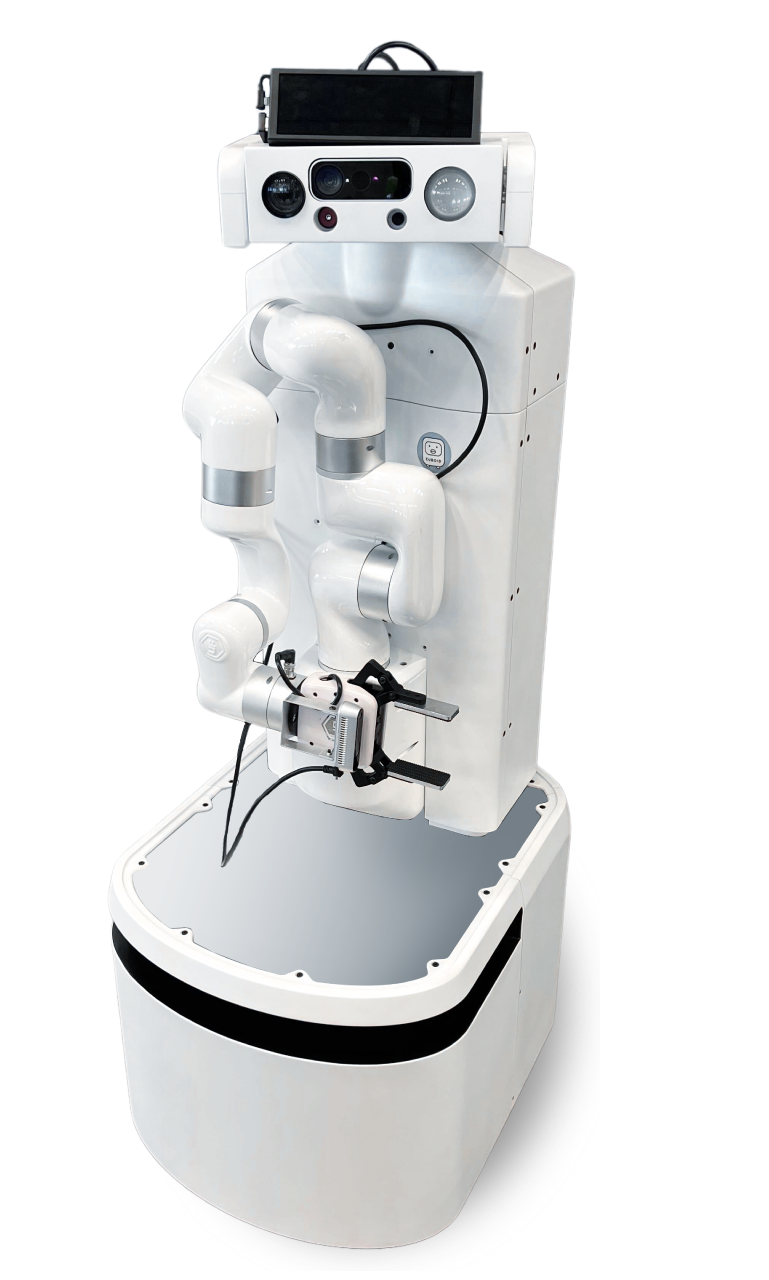
\includegraphics[width=0.4\textwidth]{images/soar.png}
	%\caption{Robot SOAR}%
	\label{fig:soar}
\end{wrapfigure}

Specifications are as follows:

\begin{itemize}
	\item Base: differential drive, 0.83 m/s max speed.
	\item Dimensions: (w) 550 mm (d) 650 mm (h) 1360 mm - 1770 mm
	\item Weight: 92 kg
	\item Arm: 8 DOF (1 DOF torso, 7 DOF manipulator)
	\item Sensors:
	      \begin{itemize}
		      \item Mobile Base:
		            \begin{itemize}
			            \item Hinson LE-50621 LiDAR
			            \item N100 9-axis IMU
		            \end{itemize}
		      \item Head:
		            \begin{itemize}
			            \item Azure Kinect RGB-D camera
			            \item ECM-SP10 microphone
			            \item JM800S-30-360X zoom camera
			            \item Seek Thermal CompactPRO Fast Frame
		            \end{itemize}
		      \item Arm:
		            \begin{itemize}
			            \item Realsense D435 RGB-D camera
		            \end{itemize}
	      \end{itemize}
	\item PC: Intel NUC (NUC11PHKi7C)
	\item Display: THANKO C-79D21B
	\item Speaker: YAMAHA VXS1MLB
\end{itemize}

\section*{SOAR Software Description}
% Please describe in this section the software you are using to control your robot. Consider the following example:

SOAR use the following software components:

\begin{itemize}
	\item Platform: Ubuntu 20.04 ROS Noetic
	\item Navigation: ROS Navigation Stack, EBand local planner
	\item Arm Motion Planner: MoveIt ROS package
	\item Object Recognition:
	      \begin{itemize}
		      \item YOLOv8
		      \item \text{jsk\_pcl\_ros} ROS package
	      \end{itemize}
	\item Behavior Architecture: SMACH ROS package
	\item Hotword: EfficientWord-Net
	\item Speech Recognition: Google Dialogflow
	\item Speech Generation: Google Text-To-Speech
	\item Person Recognition: \text{spencer\_people\_tracking} ROS package
\end{itemize}
